\documentclass{vldb}

\usepackage[noend]{algpseudocode}
\usepackage{algorithm}
\usepackage{balance}
\usepackage{booktabs}
\usepackage{invariantconfluence}
\usepackage{listings}
\usepackage{pervasives}
\usepackage{printlen}
\usepackage{python}
\usepackage{subcaption}
\usepackage{tikz}
\usetikzlibrary{arrows}
\usetikzlibrary{calc}
\usetikzlibrary{patterns}

\newcommand{\thetitle}{Interactive Checks for Coordination Avoidance}

% Include information below and uncomment for camera ready.
\vldbTitle{\thetitle}
\vldbAuthors{Michael Whittaker and Joseph M. Hellerstein}
\vldbDOI{https://doi.org/10.14778/3275536.3275538}
\vldbVolume{12}
\vldbNumber{1}
\vldbYear{2019}

\begin{document}
  \title{\thetitle}
  \iftoggle{techreportenabled}{\subtitle{Technical Report. \today.}}{}

  \numberofauthors{2}
  \author{
  \alignauthor
  Michael Whittaker \\
         \affaddr{UC Berkeley}\\
         \affaddr{Berkeley, CA}\\
         \email{mjwhittaker@berkeley.edu}
  \alignauthor
  Joseph M. Hellerstein \\
         \affaddr{UC Berkeley}\\
         \affaddr{Berkeley, CA}\\
         \email{hellerstein@berkeley.edu}
  }
  \date{TBD}

  \maketitle
  {\begin{abstract}
Strongly consistent distributed systems are easy to reason about but face
fundamental limitations in availability and performance. Weakly consistent
systems can be implemented with very high performance but place a burden on the
application developer to reason about complex interleavings of execution.
\Invariantconfluence{} provides a formal framework for understanding when we
can get the best of both worlds. An \invariantconfluent{} object can be
efficiently replicated with no coordination needed to preserve its invariants.
However, actually determining whether or not an object is \invariantconfluent{}
is challenging.

In this paper, we establish conditions under which a commonly used sufficient
condition for \invariantconfluence{} is both necessary and sufficient, and we
use this condition to design a general-purpose interactive
\invariantconfluence{} decision procedure. We then take a step beyond
\invariantconfluence{} and introduce a generalization of
\invariantconfluence{}, called segmented \invariantconfluence{}, that allows us
to replicate non-\invariantconfluent{} objects with a small amount of
coordination. We implement these formalisms in a prototype called Lucy and
find that our decision procedures efficiently handle common real-world
workloads including foreign keys, escrow transactions, and more.
\end{abstract}
}

  % Force a column break so that the introduction section title isn't by itself
  % at the bottom of the first column.
  \vfill\null

  {\section{Introduction}
When an application designer decides to replicate a piece of data, they have to
make a fundamental choice between weak and strong consistency. Replicating the
data with strong consistency using a technique like distributed transactions
(e.g., \cite{bernstein1981concurrency,mohan1986transaction}) or state machine
replication (e.g., \cite{schneider1990implementing, lamport1998part,
liskov2012viewstamped, ongaro2014search}) makes the application designer's life
very easy. To the developer, a strongly consistent system behaves exactly like
a single-threaded system running on a single node, so reasoning about the
behavior of the system is simple~\cite{herlihy1990linearizability}.
Unfortunately, strong consistency is at odds with performance. The CAP theorem
and PACELC theorem tell us that strongly consistent systems suffer from higher
latency at best and unavailability at worst~\cite{gilbert2002brewer,
brewer2012cap, abadi2012consistency}. On the other hand, weak consistency
models like eventual consistency~\cite{vogels2009eventually}, PRAM
consistency~\cite{lipton1988pram}, causal consistency~\cite{ahamad1995causal},
and others~\cite{lloyd2011don, mehdi2017can} allow data to be replicated with
high availability and low latency, but they put a tremendous burden on the
application designer to reason about the complex interleavings of operations
that are allowed by these weak consistency models. In particular, weak
consistency models strip an application developer of one of the earliest and
most effective tools that is used to reason about the execution of programs:
application invariants~\cite{hoare1969axiomatic, balegas2015towards} such as
database integrity constraints~\cite{grefen1993integrity, gupta1993local}. Even
if every transaction executing in a weakly consistent system individually
maintains an application invariant, the system as a whole can produce
invariant-violating states.

Is it possible for us to have our strongly consistent cake and eat it with high
availability too? Can we replicate a piece of data with weak consistency but
still ensure that its invariants are maintained? Yes... sometimes. Bailis et
al.\ introduced the notion of \emph{\invariantconfluence{}} as a necessary and
sufficient condition for when invariants can be maintained over replicated data
without the need for any coordination~\cite{bailis2014coordination}. If an
object is \invariantconfluent{} with respect to an invariant, we can replicate
it with the performance benefits of weak consistency and (some of) the
correctness benefits of strong consistency.

Unfortunately, to date, the task of identifying whether or not an object
actually is \invariantconfluent{} has remained an exercise in human proof
generation. Bailis et al.\ manually categorized a set of common objects,
transactions, and invariants (e.g.\ foreign key constraints on relations,
linear constraints on integers) as \invariantconfluent{} or not. Hand-written
proofs of this sort are unreasonable to expect from programmers. Ideally we
would have a general-purpose program that can automatically determine
\invariantconfluence{} for us.  \textbf{The first main thrust of this paper is
to make \invariantconfluence{} checkable:} to design a general-purpose
\invariantconfluence{} decision procedure, and implement it in an interactive
system.

Unfortunately, designing such a general-purpose decision procedure is
impossible because determining the \invariantconfluence{} of an object is
undecidable in general. Still, we can develop a decision procedure that works
well in the common case.
%
For example, many prior efforts have developed decision procedures for
\emph{\invariantclosure{}}, a sufficient (but not necessary) condition for
\invariantconfluence{}~\cite{li2012making, li2014automating}. The existing
approaches check whether an object is \invariantclosed{}. If it is, then they
conclude that it is also \invariantconfluent{}. If it's not, then the current
approaches are unable to conclude anything about whether or not the object is
\invariantconfluent{}.

In this paper, we take a step back and study the underlying reason \emph{why}
\invariantclosure{} is not necessary for \invariantconfluence{}.
%
% We find that \invariantconfluence{} is fundamentally a reachability property,
% checking whether certain values of our replicated object can actually be
% obtained in the execution of a system. We discover that unreachable, yet
% invariant satisfying, states cause \invariantclosure{} to be an unnecessary
% condition.
%
Using this understanding, we construct a set of modest conditions under which
\invariantclosure{} and \invariantconfluence{} are in fact \emph{equivalent},
allowing us to reduce the problem of determining \invariantconfluence{} to that
of determining \invariantclosure{}.
%
Then, we use these conditions to design a general-purpose interactive
\invariantconfluence{} decision procedure and a new sufficient condition for
\invariantconfluence{}, dubbed \emph{\mergereducibility}. \Mergereducibility{}
covers some cases that are not covered by \invariantclosure{}, and it can be
checked automatically.

% Then, we use these conditions to design a general-purpose interactive
% \invariantconfluence{} decision procedure. Users iteratively interact with the
% decision procedure, eliminating unreachable states from the invariant, moving
% towards the conditions under which \invariantclosure{} and
% \invariantconfluence{} are equivalent. Meanwhile, the decision procedure
% generates examples of reachable and unreachable states which help the user
% recognize patterns that describe reachability. We also leverage our intuitions
% about reachability to develop a new sufficient condition for
% \invariantconfluence{}, dubbed \emph{\mergereducibility}. \Mergereducibility{}
% covers some cases that are not covered by \invariantclosure{}, and it can be
% automatically checked without any user interaction.

\textbf{The second main thrust of this paper is to partially avoid coordination
even in programs that require it}, by generalizing \invariantconfluence{} to a
property called \emph{segmented \invariantconfluence{}}. While
\invariantconfluence{} characterizes objects that can be replicated
\emph{without any} coordination, segmented \invariantconfluence{} allows us to
replicate non-\invariantconfluent{} objects with only \emph{occasional}
coordination. The main idea is to divide the set of invariant-satisfying states
into \emph{segments}, with a restricted set of transactions allowed in each
segment.  Within a segment servers act without any coordination; they
synchronize only to transition across segment boundaries. This design
highlights the trade-off between application complexity and
coordination-freedom; more complex applications require more segments which
require more coordination, and vice-versa.

Finally, we present Lucy: an implementation of our decision procedures and a
system for replicating \invariantconfluent{} and segmented
\invariantconfluent{} objects. Using Lucy, we find that our decision
procedures can efficiently handle a wide range of common workloads. For
example, in \secref{Evaluation}, we apply Lucy to foreign key constraints,
escrow transactions, an auction application, and the TPC-C benchmark. Lucy
processes these workloads in less than half a second, and no workload requires
more than 66 lines of code to specify. Moreover, we find that segmented
\invariantconfluent{} replication can achieve 10x to 100x more throughput than
linearizable replication for low-coordination workloads.

In closing, here is an outline of the paper and of our contributions:
%
We propose a novel expression-oriented definition of \invariantconfluence{}
that is both formal and simple (\secref{InvariantConfluence}).
%
We develop an understanding of why \invariantclosure{} is not necessary for
\invariantconfluence{} and use this understanding to develop conditions under
which it is both necessary and sufficient (\secref{InvariantClosure}).
%
We exploit these conditions to design a general-purpose interactive decision
procedure for \invariantconfluence{} (\secref{InteractiveDecisionProcedure}).
%
We again exploit these conditions to design a novel non-trivial sufficient
condition for \invariantconfluence{}, called \mergereducibility.
%
We present segmented \invariantconfluence{}: a generalization of
\invariantconfluence{} that uses a small amount of coordination to maintain
invariants for replicated objects that are otherwise not \invariantconfluent{}
(\secref{SegmentedInvariantConfluence}).
%
We evaluate our methods using a prototype implementation called Lucy
(\secref{Evaluation}).
}
  {\section{Invariant Confluence}\seclabel{InvariantConfluence}
Informally, a replicated object is \defword{\invariantconfluent{}} with respect
to an invariant if every replica of the object is guaranteed to satisfy the
invariant despite the possibility of different replicas being concurrently
modified or merged together~\cite{bailis2014coordination}. In this section, we
make this informal notion of \invariantconfluence{} precise.

We begin by introducing our system model of replicated objects in which a
distributed object and accompanying invariant is replicated across a set of
servers. Clients send transactions to servers, and a server executes a
transaction so long as it maintains the invariant. Servers execute
transactions without coordination, but to avoid state divergence, servers
periodically gossip with one another and merge their replicas.
%
After we introduce the system model, we present a formal definition of
\invariantconfluence{}.

\subsection{System Model}

A \defword{distributed object} $O = (S, \join)$ consists of a set $S$ of states
and a binary merge operator $\join: S \times S \to S$ that merges two states
into one. A \defword{transaction} $t: S \to S$ is a
function that maps one state to another. An \defword{invariant} $I$ is a subset
of $S$. Notationally, we write $I(s)$ to denote that $s$ satisfies the
invariant (i.e. $s \in I$) and $\lnot I(s)$ to denote that $s$ does not satisfy
the invariant (i.e. $s \notin I$).

\begin{example}\examplelabel{Ints}
  $O = (\ints, \max)$ is a distributed object consisting of integers merged by the
  $\max$ function; $t(x) = x + 1$ is a transaction that adds one to a state; and
  $\setst{x \in \ints}{x \geq 0}$ is the invariant that states $x$ are
  non-negative.
\end{example}

Note that we do not assume any properties of $\join$, like associativity or
commutativity. Also note that by modelling a transaction $t$ as a function $S
\to S$, we focus exclusively on the effects that a transaction has on the
object (i.e.\ ``writes'' to the object). Transactions are also free to read the
value of the object, but these reads are not captured by our model because, as
we'll see, they do not affect \invariantconfluence{}. For example, we could
model any read-only transaction as a function $t$ where $t(s) = s$ for every $s
\in S$.

In our system model, a distributed object $O$ is replicated across a set $p_1,
\ldots, p_n$ of $n$ servers. Each server $p_i$ manages a replica $s_i \in S$ of
the replicated object. Every server begins with a start state $s_0 \in S$, a
fixed set $T$ of transactions, and an invariant $I$. Servers repeatedly perform
one of two actions.

First, a client can contact a server $p_i$ and request that it
\markrevisions{executes} a transaction $t \in T$. $p_i$ speculatively executes
$t$, transitioning from state $s_i$ to state $t(s_i)$. If $t(s_i)$ satisfies
the invariant---i.e.  $I(t(s_i))$---then $p_i$ commits the transaction and
remains in state $t(s_i)$.  Otherwise, $p_i$ aborts the transaction and reverts
to state $s_i$.

Second, a server $p_i$ can send its state $s_i$ to another server $p_j$ with
state $s_j$ causing $p_j$ to transition from state $s_j$  to state $s_i \join
s_j$. Servers periodically merge states with one another in order to keep their
states loosely synchronized\footnote{%
  Notably, if $O$ is a CRDT---i.e. $O$ is a semilattice and every transaction
  $t \in T$ is inflationary---then this periodic merging ensures that $O$ is
  strongly eventually consistent~\cite{shapiro2011conflict}.
}.
Note that unlike with transactions, servers \emph{cannot} abort a merge; server
$p_j$ must transition from $s_j$ to $s_i \join s_j$ whether or not $s_i \join
s_j$ satisfies the invariant.

Informally, $O$ is \defword{\invariantconfluent{}} with respect to $s_0$, $T$,
and $I$, abbreviated \defword{\sTIconfluent{}}, if every replica $s_1, \ldots,
s_n$ is guaranteed to always satisfy the invariant $I$ in every possible
execution of the system.

\subsection{Expression-Based Formalism}
To define \invariantconfluence{} formally, we represent a state produced by a
system execution as a simple expression generated by the grammar
%
\[
  \hfill
  e ::= s \mid t(e) \mid e_1 \join e_2
  \hfill
\]
%
where $s$ represents a state in $S$ and $t$ represents a transaction in $T$. As
an example, consider the system execution in \figref{SystemExecution} in which
a distributed object is replicated across servers $p_1$, $p_2$, and $p_3$.
Server $p_3$ begins with state $s_0$, transitions to state $s_2$ by executing
transaction $u$, transitions to state $s_5$ by executing transaction $w$, and
then transitions to state $s_7$ by merging with server $p_1$. Similarly, server
$p_1$ ends up with state $s_6$ after executing transactions $t$ and $v$ and
merging with server $p_2$. In \figref{Expression}, we see the abstract syntax
tree of the corresponding expression for state $s_7$.

{\input{figures/invariant_confluence_definitions}}

We say an expression $e$ is \defword{\sTIreachable{}} if it corresponds to a
valid execution of our system model. Formally, we define
$\sTIreachablepredicate{e}$ to be the smallest predicate that satisfies the
following equations:
\begin{itemize}
  \item
    $\sTIreachablepredicate{s_0}$.
  \item
    For all expressions $e$ and for all transactions $t$ in the set $T$ of
    transactions, if $\sTIreachablepredicate{e}$ and $I(t(e))$, then
    $\sTIreachablepredicate{t(e)}$.
  \item
    For all expressions $e_1$ and $e_2$, if $\sTIreachablepredicate{e_1}$ and
    $\sTIreachablepredicate{e_2}$, then $\sTIreachablepredicate{e_1 \join
    e_2}$.
\end{itemize}
Similarly, we say a state $s \in S$ is \sTIreachable{} if there exists an
\sTIreachable{} expression $e$ that evaluates to $s$. Returning to
\exampleref{Ints} with start state $s_0 = 42$, we see that all integers greater
than or equal to 42 (i.e.\ $\setst{x \in \ints}{x \geq 42}$) are
\sTIreachable{}, and all other integers are \sTIunreachable{}.

Finally, we say $O$ is \defword{\invariantconfluent} with respect to $s_0$,
$T$, and $I$, abbreviated \defword{\sTIconfluent{}}, if all reachable states
satisfy the invariant:
\[
  \hfill
  \setst{s \in S}{\sTIreachablepredicate{s}} \subseteq I
  \hfill
\]

\subsection{Equivalence to Existing Definition}
Our definition of \invariantconfluence{} is different than the original
definition given in~\cite{bailis2014coordination}, but the difference is merely
cosmetic. We now prove that the two definitions are equivalent.

We say an expression $e$ \defword{recursively satisfies $I$}, denoted
$\Irec{e}$, if $e$ and all of $e$'s children satisfy $I$. That is,
\begin{itemize}
  \item
    $\Irec{s}$ if $I(s)$,

  \item
    $\Irec{t(e)}$ if $\Irec{e}$ and $I(t(e))$, and

  \item
    $\Irec{e_1 \join e_2}$ if $\Irec{e_1}$, $\Irec{e_2}$, and $I(e_1 \join
    e_2)$.
\end{itemize}

In~\cite{bailis2014coordination}, Bailis et al.\ define \sTIconfluence{} to
mean that (a) the start state $s_0$ satisfies the invariant and (b) all
\sTIreachable{} expressions recursively satisfying $I$ are closed under join.
That is, $O$ is \sTIconfluent{} if $I(s_0)$ and
\begin{gather*}
  \hspace{0.75in} \forall e_1, e_2 \in \setst{e}{\sTIreachablepredicate{e}}.\; \\
  \hspace{0.75in} \Irec{e_1} \land \Irec{e_2} \implies I(e_1 \join e_2)
\end{gather*}

\begin{theorem}\thmlabel{TwoIconfluenceDefs}
  Consider a state based object $O = (S, \join)$, a start state $s_0$, a set of
  transactions $T$, and an invariant $I$. The following two are equivalent:
  \begin{enumerate}
    \item
      $\setst{s \in S}{\sTIreachablepredicate{s}} \subseteq I$

    \item
      $I(s_0)$ and
      $\forall e_1, e_2 \in \setst{e}{\sTIreachablepredicate{e}}.\;
         \Irec{e_1} \land \Irec{e_2} \implies I(e_1 \join e_2)$
  \end{enumerate}
\end{theorem}
\begin{proof}
  First, we show that (1) implies (2). Trivially,
  $\sTIreachablepredicate{s_0}$, so by (1), $I(s_0)$. Let $e_1$ and $e_2$ be
  arbitrary \sTIreachable{} expressions. Then $e_1 \join e_2$ is also
  reachable, so by (1), $I(e_1 \join e_2)$.

  Next, we show that (2) implies (1). We prove by structural induction that for
  all $e$, $\sTIreachablepredicate{e} \implies \Irec{e}$. From this, (1) is
  immediate.
  \begin{itemize}
    \item \textbf{Case $s_0$.}
      $I(s_0)$ by (2), so $\Irec{s_0}$

    \item \textbf{Case $t(e)$.}
      Let $t(e)$ be \sTIreachable{}. Then, $\sTIreachablepredicate{e}$ and
      $I(t(e))$. By the inductive hypothesis, $\Irec{e}$, so by the definition
      of $\Irec{\cdot}$, $\Irec{t(e)}$.

    \item \textbf{Case $e_1 \join e_2$.}
      Let $e_1 \join e_2$ be \sTIreachable{}. Then,
      $\sTIreachablepredicate{e_1}$ and $\sTIreachablepredicate{e_2}$. By the
      inductive hypothesis, $\Irec{e_1}$ and $\Irec{e_2}$. By $(2)$, $I(e_1
      \join e_2)$. Thus, by the definition of $\Irec{\cdot}$, $\Irec{e_1 \join
      e_2}$.
  \end{itemize}
\end{proof}
}
  {\section{Invariant-Closure}
% - define invariant-closure and introduce it as a sufficient condition
% - cite existing work to show that people have used invariant closure to
%   reason about invariant-confluence
% - explain why invariant closure can fail and why its not sufficient using the
%   two-integers example
% - state main theorem

}
  {\section{An Interactive Decision Procedure}
% - describe how main theorem gives us intution about interactive dp
% - present the algorithm
% - walk through an example
% - describe how the algorithm is robust to errors
}
  {\section{Merge Reduction}\seclabel{MergeReduction}
In \secref{InvariantClosure}, we discussed how \invariantconfluence{} is
fundamentally a property of reachability and that \invariantclosure{} is
sufficient but not necessary for \invariantconfluence{} because it fails to
incorporate any notion of reachability. Using this intuition, we established
\thmref{IclosureEquivalentIconfluence} and then exploited the theorem in
\algoref{InteractiveDecisionProcedure}. In this section, we again take
advantage of this intuition to develop a new sufficient condition for
\invariantconfluence{} that can be checked without user interaction and that
covers some cases not covered by \invariantclosure{}.

An expression $e = t_1(t_2(\ldots(t_n(s))\ldots))$ is \defword{merge-free} if
does not contain any merges (i.e.\ it is generated by the grammar $e ::= s \mid
t(e)$). An object $O = (S, \join)$ is \defword{merge-reducible} with respect to
a start state $s_0 \in S$, a set of transactions $T$, and an invariant $I$,
abbreviated \defword{\sTImergereducible}, if for every pair $e_1$ and $e_2$ of
merge-free \sTIreachable{} expressions, there exists some merge-free
\sTIreachable{} expression $e_3$ that evaluates to the same state as $e_1 \join
e_2$. Intuitively, if $O$ is merge-reducible, we can replace $e_1 \join e_2$
(which has one merge) with $e_3$ (which has no merges) to obtain an equivalent
expression with fewer merges.

\begin{example}\examplelabel{MergeReducible}
  Consider the distributed object $O = (\ints, \max)$ consisting of integers
  merged by the max function. Our start state $s_0 = 0$ and our invariant
  $I = \setst{x \in \ints}{x \geq 0}$. Our set $T$ of transactions is the
  infinite set $T = \setst{t_y}{y \in \ints}$ where $t_y(x) = x + y$ is a
  transaction that adds $y$ to the state. For example, $t_2$ is a transaction
  that adds $2$ to the state, and $t_{-3}$ is a transaction which subtracts $3$
  from the state.
  %
  $O$ is \sTImergereducible{}. Consider two merge-free \sTIreachable{}
  expressions $e_1$ and $e_2$ that evaluate to states $x_1$ and $x_2$. Without
  loss of generality, assume $x_1 \geq x_2$. Then, we can replace $e_1 \join
  e_2$ (which evaluates to $x_1$) with $e_1$. We can also replace it with
  $t_{x_1}(0)$.
\end{example}

\begin{example}\examplelabel{NotMergeReducible}
  Consider the distributed object $O = (\set{X \subseteq \ints}, \join)$ in
  which each state is a set of integers and where $X_1 \join X_2 = \set{y}$
  where $y = \sum_{x \in X_1} x + \sum_{x \in X_2} x$. Our start state state
  $s_0 = \emptyset{}$ and our invariant $I = \setst{X}{\forall x \in X.\ x \
  \text{is even}}$. Our set $T$ of transactions is the set $T = \set{t_0, t_2,
  t_4}$ where $t_i(X) = X \cup \set{i}$ is a transaction that adds $i$ to the
  state. For example, $t_2(\set{0}) = \set{0, 2}$.
  %
  $O$ is \emph{not} \sTImergereducible{}. Consider the two merge-free
  \sTIreachable{} expressions $e_1 = t_2(\emptyset)$ and $e_2 =
  t_4(\emptyset)$. $e_1 \join e_2$ evaluates to $\set{6}$, but there does not
  exist a merge-free expression that evaluates to $\set{6}$.
\end{example}

{\begin{figure*}[ht]
  \centering

  \tikzstyle{s0color}=[fill=flatred]
  \tikzstyle{s1color}=[fill=flatgreen]
  \tikzstyle{s2color}=[fill=flatdenim]
  \tikzstyle{s3color}=[fill=flatorange]
  \tikzstyle{s4color}=[fill=flatyellow]
  \tikzstyle{s5color}=[fill=flatcyan]
  \tikzstyle{s6color}=[fill=flatpurple]
  \tikzstyle{s7color}=[fill=flatblue]
  \tikzstyle{astedge}=[thick]
  \tikzstyle{phantomstate}=[%
    shape=circle, inner sep=2pt, draw=white, line width=1pt, fill=white]
  \tikzstyle{state}=[%
    shape=circle, inner sep=2pt, draw=black, line width=1pt, text opacity=1,
    fill opacity=0.6]
  \newcommand{\internaltext}[1]{$\boldsymbol #1$}

  \begin{tikzpicture}[xscale=1.1]
    \begin{scope}[]
                         \node[state, s7color, label={[label distance=-0.1cm] 90:$s_7$}] (s7) at (0, 0) {\internaltext{\join}};
      \draw (s7)++(210:1) node[state, s3color, label={[label distance=-0.1cm] 90:$s_3$}] (s3)           {\internaltext{\join}};
      \draw (s7)++(-30:1) node[state, s6color, label={[label distance=-0.1cm] 90:$s_6$}] (s6)           {\internaltext{\join}};
      \draw (s3)++(240:1) node[state, s1color, label={[label distance=-0.2cm] 120:$s_1$}](s1)           {\internaltext{t}};
      \draw (s3)++(-60:1) node[state, s2color, label={[label distance=-0.2cm] 60:$s_2$}] (s2)           {\internaltext{u}};
      \draw (s6)++(240:1) node[state, s4color, label={[label distance=-0.2cm] 240:$s_4$}](s4)           {\internaltext{v}};
      \draw (s6)++(-60:1) node[state, s5color, label={[label distance=-0.2cm] 60:$s_5$}] (s5)           {\internaltext{w}};
      \draw (s1)++(-90:1) node[state, s0color]                                           (n1)           {\internaltext{s_0}};
      \draw (s2)++(-90:1) node[state, s0color]                                           (n2)           {\internaltext{s_0}};
      \draw (s4)++(-90:1) node[state, s0color]                                           (n4)           {\internaltext{s_0}};
      \draw (s5)++(-90:1) node[state, s0color]                                           (n5)           {\internaltext{s_0}};
      \draw[astedge] (s7) to (s3) to (s1) to (n1);
      \draw[astedge] (s7) to (s3) to (s2) to (n2);
      \draw[astedge] (s7) to (s6) to (s4) to (n4);
      \draw[astedge] (s7) to (s6) to (s5) to (n5);
      \coordinate (A) at (s5);
    \end{scope}
    \begin{scope}[xshift=125]
      \node[state, s7color, label={[label distance=-0.1cm] 90:$s_7$}] (s7) at (0, 0) {\internaltext{\join}};
      \draw (s7)++(210:1) node[state, s3color, label={[label distance=-0.1cm] 90:$s_3$}] (s3)           {\internaltext{p}};
      \draw (s7)++(-30:1) node[state, s6color, label={[label distance=-0.1cm] 90:$s_6$}] (s6)           {\internaltext{\join}};
      \draw (s6)++(240:1) node[state, s4color, label={[label distance=-0.2cm] 240:$s_4$}](s4)           {\internaltext{v}};
      \draw (s6)++(-60:1) node[state, s5color, label={[label distance=-0.2cm] 60:$s_5$}] (s5)           {\internaltext{w}};
      \draw (s3)++(-90:1) node[state, s0color]                                           (n3)           {\internaltext{s_0}};
      \draw (s4)++(-90:1) node[state, s0color]                                           (n4)           {\internaltext{s_0}};
      \draw (s5)++(-90:1) node[state, s0color]                                           (n5)           {\internaltext{s_0}};
      \draw[astedge] (s7) to (s3) to (n3);
      \draw[astedge] (s7) to (s6) to (s4) to (n4);
      \draw[astedge] (s7) to (s6) to (s5) to (n5);
    \end{scope}
    \begin{scope}[xshift=250]
      \node[state, s7color, label={[label distance=-0.1cm] 90:$s_7$}] (s7) at (0, 0) {\internaltext{\join}};
      \draw (s7)++(210:1) node[state, s3color, label={[label distance=-0.1cm] 90:$s_3$}] (s3)           {\internaltext{p}};
      \draw (s7)++(-30:1) node[state, s6color, label={[label distance=-0.1cm] 90:$s_6$}] (s6)           {\internaltext{q}};
      \draw (s3)++(-90:1) node[state, s0color]                                           (n3)           {\internaltext{s_0}};
      \draw (s6)++(-90:1) node[state, s0color]                                           (n6)           {\internaltext{s_0}};
      \draw[astedge] (s7) to (s3) to (n3);
      \draw[astedge] (s7) to (s6) to (n6);
    \end{scope}
    \begin{scope}[xshift=350]
                         \node[state, s7color, label={[label distance=-0.1cm] 90:$s_7$}] (s7) at (0, 0) {\internaltext{r}};
      \draw (s7)++(-90:1) node[state, s0color]                                           (n7)           {\internaltext{s_0}};
      \draw[astedge] (s7) to (n7);
    \end{scope}

    \draw[-latex, line width=3pt] (A) ++ (0.55, 0) to ++(1, 0);
    \draw[-latex, line width=3pt] (A) ++ (5, 0) to ++(1, 0);
    \draw[-latex, line width=3pt] (A) ++ (9, 0) to ++(1, 0);
  \end{tikzpicture}

  \caption{%
    An illustration of the proof of \thmref{ReducibilityImpliesIconfluence}. We
    begin with a reachable expression and convert it into a merge-free
    reachable expression by repeatedly replacing the merge of two merge-free
    reachable subexpressions with an equivalent merge-free reachable
    expression. In this example, we first replace $t(s_0) \join u(s_0)$ with
    $p(s_0)$. We then replace $v(s_0) \join w(s_0)$ with $q(s_0)$. Finally, we
    replace $p(s_0) \join q(s_0)$ with $r(s_0)$.
  }\figlabel{MergingDiagram}
\end{figure*}
}

\begin{theorem}\thmlabel{ReducibilityImpliesIconfluence}
  Given an object $O = (S, \join)$, a start state $s_0 \in S$, a set of
  transactions $T$, and an invariant $I$, if $I(s_0)$ and if $O$ is
  \sTImergereducible{}, then $O$ is \sTIconfluent{}.
\end{theorem}

\begin{proof}
  Intuitively, the proof of \thmref{ReducibilityImpliesIconfluence} is a
  straightforward induction. We begin with an \sTIreachable{} expression $e$
  and repeatedly replace any subexpression that merges two merge-free
  subexpressions with an equivalent merge-free reachable subexpression (which
  we can do because $O$ is merge-reducible). We repeat this process until $e$
  has been completely replaced with an equivalent merge-free reachable
  expression $e'$. Because $I(s_0)$ and because our system model only executes
  transactions that preserve the invariant, $e'$ (and hence $e$) is guaranteed
  to satisfy the invariant. Thus, all reachable states satisfy the invariant,
  so $O$ is \invariantconfluent{}. An illustration of this idea is given in
  \figref{MergingDiagram}.

  More formally, we prove by structural induction on $e$, that for all
  \sTIreachable{} expressions $e$, there exists a merge-free \sTIreachable{}
  expression $e'$ such that $eval(e) = eval(e')$.
  \begin{itemize}
    \item \textbf{Case 1: $e = s_0$.}
      Trivially, $e' = s_0$.

    \item \textbf{Case 2: $e = t(e_1)$.}
      $e_1$ is \sTIreachable{}, so by the inductive hypothesis, there exists a
      merge-free \sTIreachable{} expression $e_1'$ such that $eval(e_1) =
      eval(e_1')$. $t(e_1)$ is \sTIreachable{}, so $I(t(e_1))$. Because
      $eval(e_1) = eval(e_1')$, we know also that $I(t(e_1'))$. Thus, $t(e_1')$
      is \sTIreachable{} (and join free), so we can let $e' = t(e_1')$.

    \item \textbf{Case 3: $e = e_1 \join e_2$.}
      $e_1$ and $e_2$ are \sTIreachable{}, so by the inductive hypothesis,
      there exists equivalent merge-free \sTIreachable{} expressions $e_1'$ and
      $e_2'$. $O$ is \sTImergereducible{}, so there exists an equivalent
      merge-free \sTIreachable{} expression $e'$.
  \end{itemize}

  Consider an arbitrary \sTIreachable{} expression $e$ and it's equivalent
  merge-free \sTIreachable{} counterpart $e'$. $e'$ is either $s_0$ or
  $t(e'')$.  In either case, it satisfies the invariant, so $O$ is
  \sTIconfluent{}.
\end{proof}

Note that while merge-reducibility is a sufficient condition for
\invariantconfluence{}, it is not necessary. The object in
\exampleref{NotMergeReducible} is \invariantconfluent{} but not
merge-reducible.

Merge-reducibility is a sufficient condition for \invariantconfluence{}, but
unlike with \invariantclosure{}, it is not straightforward to automatically
determine if an object is merge-reducible. In \thmref{LatticeProperty}, we
outline a sufficient condition for merge-reducibility that is straightforward
to determine automatically.

\begin{theorem}\thmlabel{LatticeProperty}
  Given an object $O = (S, \join)$, a start state $s_0 \in S$, a set of
  transactions $T$, and an invariant $I$, if the following criteria are met,
  then $O$ is \sTImergereducible{} (and therefore \sTIconfluent{}).
  \begin{enumerate}
    \item
      $O$ is a join-semilattice. That is, $\join$ is associative ($(x \join y)
      \join z = x \join (y \join z)$), commutative ($x \join y = y \join x$),
      and idempotent ($x \join x = x$).

    \item
      For every $t \in T$, there exists some $s_t \in S$ such that for all $s
      \in S$, $t(s) = s \join s_t$. That is, every transaction $t$ is of the
      form $t(s) = s \join s_t$ for some constant $s_t$.

    \item
      For every pair of transactions $t_1, t_2 \in T$ and for all states $s \in
      S$, if $I(s)$, $I(t_1(s))$, and $I(t_2(s))$, then $I(t_1(s) \join
      t_2(s))$.

    \item
      $I(s_0)$.
  \end{enumerate}
\end{theorem}

\newcommand{\bart}[1]{\overline{t_{#1}}}
\newcommand{\baru}[1]{\overline{u_{#1}}}
\newcommand{\bartu}[2]{\bart{#1}(\baru{#2}(s_0))}
\begin{proof}
  Let
  \[
    \hfill
    e_1 = t_n(t_{n-1}(\ldots (t_1(s_0))\ldots))
    \hfill
  \]
  and
  \[
    \hfill
    e_2 = u_m(u_{m-1}(\ldots (u_1(s_0))\ldots))
    \hfill
  \]
  be two arbitrary merge-free \sTIreachable{} expressions.
  For ease of notation, let
  \[
    \hfill
    \bart{i} = t_i(\ldots(t_1(s_0))\ldots)
    \quad\text{and}\quad
    \baru{j} = u_j(\ldots(u_1(s_0))\ldots)
    \hfill
  \]
  We want to show that there exists some merge-free \sTIreachable{} expression
  that is equivalent to $e_1 \join e_2$.
  %
  To do so, we prove by strong induction on $k \in \nats$ that if $k = i + j$
  where $0 \leq i \leq n$ and $0 \leq j \leq m$, $\bartu{i}{j}$ is
  \sTIreachable{} and $eval(\bartu{i}{j}) = eval(\bart{i}(s_0) \join
  \baru{j}(s_0))$.
  \begin{itemize}
    \item \textbf{Case $k = 0$.}
      $i = j = 0$, so $\bartu{0}{0} = s_0$ which is trivially \sTIreachable{}
      and equivalent to $\bart{0}(s_0) \join \baru{0}(s_0) = s_0 \join s_0$
      which evaluates to $s_0$ (because $\join$ is idempotent).

    \item \textbf{Case $k = 1$.}
      Without loss of generality, assume $i = 1$ and $j = 0$. Then,
      $
        \bartu{1}{0} = t_1(s_0)
      $ which is \sTIreachable{} because it is a subexpression of $\bart{n}$
      which is \sTIreachable{}. Moreover, it is equivalent to $\bart{1}(s_0)
      \join \baru{0}(s_0) = t_1(s_0) \join s_0$ which evaluates to $s_{t_1}
      \join s_0 \join s_0 = s_{t_1} \join s_0 = t_1(s_0)$ for some $s_{t_1} \in
      S$.

    \item \textbf{Case $k \geq 2$.}
      If $i = 0$, then $j = k$ and $\baru{k}(s_0)$ is \sTIreachable{} because
      it is a subexpression of $\baru{m}(s_0)$. Also, it is equivalent to
      $\bart{0}(s_0) \join \baru{k}(s_0)$ which evaluates to $\baru{k}(s_0)$.
      %
      The symmetric result holds if $j = 0$.

      Otherwise, $i, j > 1$. Let
      \begin{align*}
        e_{i-1,j-1} &= \bartu{i-1}{j-1} \\
        e_{i,j-1} &= \bartu{i}{j-1} \\
        e_{i-1,j} &= \bartu{i-1}{j}
      \end{align*}
      By the inductive hypothesis, $e_{i-1,j-1}$, $e_{i,j-1}$, and $e_{i-1,j}$
      are all \sTIreachable{}. By condition 3 (with $s = eval(e_{i-1,j-1})$,
      $t_1$ = $t_i$, and $t_2 = u_j$), $I(e_{i,j-1} \join e_{i-1,j})$.
      $e_{i,j-1} \join e_{i-1,j} = t_i(e_{i-1,j}) = u_j(e_{i,j-1}) =
      \bartu{i}{j}$, so $I(\bartu{i}{j})$. Therefore, $\bartu{i}{j}$ is
      \sTIreachable{}.
  \end{itemize}
\end{proof}

{\begin{figure}[t]
  \centering
  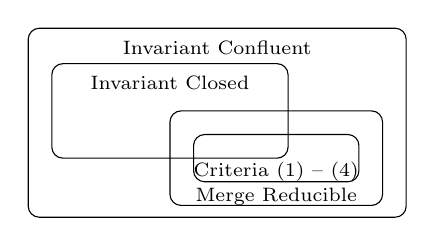
\begin{tikzpicture}[scale=0.3]
    \draw[rounded corners] (0, 0) rectangle (16, 8);
    \draw[rounded corners] (1, 2.5) rectangle (11, 6.5);
    \draw[rounded corners] (6, 0.5) rectangle (15, 4.5);
    \draw[rounded corners] (7, 1.5) rectangle ++(7, 2);
    \node[inner sep=0pt, anchor=north] at (8, 7.5) {\scriptsize Invariant Confluent};
    \node[inner sep=0pt, anchor=north] at (6, 6) {\scriptsize Invariant Closed};
    \node[inner sep=0pt, anchor=south] at (10.5, 1.5) {\scriptsize Criteria (1) -- (4)};
    \node[inner sep=0pt, anchor=south] at (10.5, 0.5) {\scriptsize Merge Reducible};
  \end{tikzpicture}
  \caption{%
    The relationship between \invariantclosure{}, \mergereducibility{},
    criteria (1) -- (4) from \thmref{LatticeProperty}, and
    \invariantconfluence{}.
  }\figlabel{IclosureVsReducible}
\end{figure}
}
{% Implication.
\tikzstyle{impl}=[-implies, double distance=3pt]

% Transaction.
\tikzstyle{txn}=[thick, -latex]

% Dashed transaction.
\tikzstyle{dtxn}=[thick, -latex, dashed]

% G transaction.
\tikzstyle{gtxn}=[thick, -latex, decorate, decoration={zigzag}]

% Dashed G transaction.
\tikzstyle{dgtxn}=[thick, -latex, densely dashed, decorate, decoration={zigzag}]

% Invariant node.
\newcommand{\inode}[3][]{
  \node[draw, shape=circle, minimum width=0.4cm] (#2) at (#3) {};
  \node[fill, shape=circle, #1] () at (#3) {};
}

% Normal node.
\newcommand{\nnode}[3][]{
  \node[fill, shape=circle, #1] (#2) at (#3) {};
}

\newcommand{\baseedges}{
  \begin{scope}[on background layer]
    \draw[txn] (03) -- (13) node[midway, above]{$u_1$};
    \draw[txn] (13) -- (23) node[midway, above]{$u_2$};
    \draw[txn] (23) -- (33) node[midway, above]{$u_3$};
    \draw[txn] (03) -- (02) node[midway, left]{$t_1$};
    \draw[txn] (02) -- (01) node[midway, left]{$t_2$};
    \draw[txn] (01) -- (00) node[midway, left]{$t_3$};
    \draw[dtxn] (00) -- (30);
    \draw[dtxn] (33) -- (30);
  \end{scope}
}

\begin{figure*}[ht]
  \centering
  \newcommand{\onescale}{1}

  \begin{subfigure}[b]{0.24\textwidth}
    \centering
    \begin{tikzpicture}[scale=\onescale]
      \foreach \x/\y in {
             1/3, 2/3, 3/3,
        0/2,
        0/1,
        0/0%
      } {
        \inode{\x\y}{\x, \y}
      }
      \foreach \x/\y in {0/3} {
        \inode[flatred]{\x\y}{\x, \y}
      }
      \nnode{30}{3, 0}
      \baseedges{}
    \end{tikzpicture}
    \caption{$k=0$}
    \label{fig:one-is-enough-base}
  \end{subfigure}
  \begin{subfigure}[b]{0.24\textwidth}
    \centering
    \begin{tikzpicture}[scale=\onescale]
      \foreach \x/\y in {
        0/3,      2/3, 3/3,
        %
        0/1,
        0/0%
      } {
        \inode{\x\y}{\x, \y}
      }
      \foreach \x/\y in {0/2, 1/3} {
        \inode[flatred]{\x\y}{\x, \y}
      }
      \nnode{30}{3, 0}
      \baseedges{}
    \end{tikzpicture}
    \caption{$k=1$}
    \label{}
  \end{subfigure}%
  \begin{subfigure}[b]{0.24\textwidth}
    \centering
    \begin{tikzpicture}[scale=\onescale]
      \foreach \x/\y in {
        0/3, 1/3,      3/3,
        0/2,
        %
        0/0%
      } {
        \inode{\x\y}{\x, \y}
      }
      \foreach \x/\y in {0/1, 1/2, 2/3} {
        \inode[flatred]{\x\y}{\x, \y}
      }
      \nnode{30}{3, 0}
      \baseedges{}
      \draw[txn] (02) -- (12) node[midway, above] {$u_1$};
      \draw[txn] (13) -- (12) node[midway, left]  {$t_1$};
    \end{tikzpicture}
    \caption{$k=2$}
    \label{}
  \end{subfigure}%
  \begin{subfigure}[b]{0.24\textwidth}
    \centering
    \begin{tikzpicture}[scale=\onescale]
      \foreach \x/\y in {
        0/3, 1/3, 2/3,
        0/2, 1/2,
        0/1%
        %
      } {
        \inode{\x\y}{\x, \y}
      }
      \foreach \x/\y in {0/0, 1/1, 2/2, 3/3} {
        \inode[flatred]{\x\y}{\x, \y}
      }
      \nnode{30}{3, 0}
      \baseedges{}
      \draw[txn] (02) -- (12) node[midway, above] {$u_1$};
      \draw[txn] (13) -- (12) node[midway, left]  {$t_1$};
      \draw[txn] (01) -- (11) node[midway, above] {$u_1$};
      \draw[txn] (12) -- (11) node[midway, left]  {$t_2$};
      \draw[txn] (12) -- (22) node[midway, above] {$u_2$};
      \draw[txn] (23) -- (22) node[midway, left]  {$t_1$};
    \end{tikzpicture}
    \caption{$k=3$}
    \label{}
  \end{subfigure}

  \begin{subfigure}[b]{0.3\textwidth}
    \centering
    \begin{tikzpicture}[scale=\onescale]
      \foreach \x/\y in {
        0/3, 1/3, 2/3, 3/3,
        0/2, 1/2, 2/2,
        0/1, 1/1,
        0/0%
      } {
        \inode{\x\y}{\x, \y}
      }
      \foreach \x/\y in {1/0, 2/1, 3/2} {
        \inode[flatred]{\x\y}{\x, \y}
      }
      \nnode{30}{3, 0}
      \baseedges{}
      \draw[txn] (02) -- (12) node[midway, above] {$u_1$};
      \draw[txn] (13) -- (12) node[midway, left]  {$t_1$};
      \draw[txn] (01) -- (11) node[midway, above] {$u_1$};
      \draw[txn] (12) -- (11) node[midway, left]  {$t_2$};
      \draw[txn] (12) -- (22) node[midway, above] {$u_2$};
      \draw[txn] (23) -- (22) node[midway, left]  {$t_1$};
      \draw[txn] (00) -- (10) node[midway, above] {$u_1$};
      \draw[txn] (11) -- (10) node[midway, left]  {$t_3$};
      \draw[txn] (11) -- (21) node[midway, above] {$u_2$};
      \draw[txn] (22) -- (21) node[midway, left]  {$t_2$};
      \draw[txn] (22) -- (32) node[midway, above] {$u_3$};
      \draw[txn] (33) -- (32) node[midway, left]  {$t_1$};
    \end{tikzpicture}
    \caption{$k=4$}
    \label{}
  \end{subfigure}%
  \begin{subfigure}[b]{0.3\textwidth}
    \centering
    \begin{tikzpicture}[scale=\onescale]
      \foreach \x/\y in {
        0/3, 1/3, 2/3, 3/3,
        0/2, 1/2, 2/2, 3/2,
        0/1, 1/1, 2/1,
        0/0, 1/0%
      } {
        \inode{\x\y}{\x, \y}
      }
      \foreach \x/\y in {2/0, 3/1} {
        \inode[flatred]{\x\y}{\x, \y}
      }
      \nnode{30}{3, 0}
      \baseedges{}
      \draw[txn] (02) -- (12) node[midway, above] {$u_1$};
      \draw[txn] (13) -- (12) node[midway, left]  {$t_1$};
      \draw[txn] (01) -- (11) node[midway, above] {$u_1$};
      \draw[txn] (12) -- (11) node[midway, left]  {$t_2$};
      \draw[txn] (12) -- (22) node[midway, above] {$u_2$};
      \draw[txn] (23) -- (22) node[midway, left]  {$t_1$};
      \draw[txn] (00) -- (10) node[midway, above] {$u_1$};
      \draw[txn] (11) -- (10) node[midway, left]  {$t_3$};
      \draw[txn] (11) -- (21) node[midway, above] {$u_2$};
      \draw[txn] (22) -- (21) node[midway, left]  {$t_2$};
      \draw[txn] (22) -- (32) node[midway, above] {$u_3$};
      \draw[txn] (33) -- (32) node[midway, left]  {$t_1$};
      \draw[txn] (10) -- (20) node[midway, above] {$u_2$};
      \draw[txn] (21) -- (20) node[midway, left]  {$t_3$};
      \draw[txn] (21) -- (31) node[midway, above] {$u_3$};
      \draw[txn] (32) -- (31) node[midway, left]  {$t_2$};
    \end{tikzpicture}
    \caption{$k=5$}
    \label{}
  \end{subfigure}%
  \begin{subfigure}[b]{0.3\textwidth}
    \centering
    \begin{tikzpicture}[scale=\onescale]
      \foreach \x/\y in {
        0/3, 1/3, 2/3, 3/3,
        0/2, 1/2, 2/2, 3/2,
        0/1, 1/1, 2/1, 3/1,
        0/0, 1/0, 2/0%
      } {
        \inode{\x\y}{\x, \y}
      }
      \inode[flatred]{30}{3, 0}
      \baseedges{}
      \draw[txn] (02) -- (12) node[midway, above] {$u_1$};
      \draw[txn] (13) -- (12) node[midway, left]  {$t_1$};
      \draw[txn] (01) -- (11) node[midway, above] {$u_1$};
      \draw[txn] (12) -- (11) node[midway, left]  {$t_2$};
      \draw[txn] (12) -- (22) node[midway, above] {$u_2$};
      \draw[txn] (23) -- (22) node[midway, left]  {$t_1$};
      \draw[txn] (00) -- (10) node[midway, above] {$u_1$};
      \draw[txn] (11) -- (10) node[midway, left]  {$t_3$};
      \draw[txn] (11) -- (21) node[midway, above] {$u_2$};
      \draw[txn] (22) -- (21) node[midway, left]  {$t_2$};
      \draw[txn] (22) -- (32) node[midway, above] {$u_3$};
      \draw[txn] (33) -- (32) node[midway, left]  {$t_1$};
      \draw[txn] (10) -- (20) node[midway, above] {$u_2$};
      \draw[txn] (21) -- (20) node[midway, left]  {$t_3$};
      \draw[txn] (21) -- (31) node[midway, above] {$u_3$};
      \draw[txn] (32) -- (31) node[midway, left]  {$t_2$};
      \draw[txn] (20) -- (30) node[midway, above] {$u_3$};
      \draw[txn] (31) -- (30) node[midway, left]  {$t_3$};
    \end{tikzpicture}
    \caption{$k=6$}
    \label{}
  \end{subfigure}

  \caption{Illustration of the proof of \thmref{LatticeProperty} for $n=m=3$}
  \figlabel{DiamondProofDiagram}
\end{figure*}
}

An illustration of this proof is given in \figref{DiamondProofDiagram}. We
arrange the expressions $e_1$ and $e_2$ as the left and top edges of a square
grid. Each point in the grid represents a state (with $s_0$ in the top left
corner), and each edge represents the application of a transaction. A state is
circled if we know it satisfies the invariant.
%
Condition (1) and (2) tell us that the order in which we apply transactions is
immaterial. Thus, if we begin at the top left of the square and walk to any
other point in the square, applying transactions along the way, it does not
matter which path we take. They are all equivalent. Condition (4) tells us that
the top-left corner satisfies the invariant. We induct to repeatedly apply
condition (3) to ``fill in'' the square, one block at a time. In iteration $k$,
we discover that all points with a Manhattan distance of $k$ from the top left
corner satisfy the invariant. Ultimately, we conclude that the bottom right
corner (i.e., $e_1 \join e_2$) satisfies the invariant and is equivalent to
$\bartu{n}{m}$.

\thmref{IclosureImpliesIconfluence} states that \invariantclosure{} is a
sufficient condition for \invariantconfluence{}, and \thmref{LatticeProperty}
states that criteria (1) -- (4) are sufficient conditions for
\invariantconfluence{}. How do these sufficient conditions relate to one
another?  Clearly, not all \invariantclosed{} objects are semilattices, so
\invariantclosure{} does not imply criteria (1) -- (4). Conversely, there are
some objects that satisfy criteria (1) -- (4) that are not
\invariantclosed{}. Here's one example.

\begin{example}\examplelabel{TwoSets}
  Let $O = (\mathcal{P}(\nats), \cup)$ where $\mathcal{P}(\nats)$ is the power
  set of the natural numbers. Our start state $s_0 = \set{0}$ is the set of
  $0$. Let $t_Y(X) = X \cup Y$ be the transaction that unions $Y$ with its
  argument $X$. Our set $T = \setst{t_Y}{Y \subseteq \nats}$ of transactions
  consists of all possible $t_Y$. Our invariant $I$ consists of all non-empty
  sets $X$ that contain only even or only odd elements. That is, $I = \setst{X
  \subseteq 2\nats}{X \neq \emptyset} \cup \setst{X \subseteq 2\nats + 1}{X
  \neq \emptyset}$.

  Criteria (1), (2), (3) and (4) are all satisfied. However, $O$ is not
  \Iclosed{}. Let $s_1 = \set{0}$ and $s_2 = \set{1}$. Then, $I(s_1)$ and
  $I(s_2)$, but letting $s_3 = s_1 \cup s_2 = \set{0, 1}$, $\lnot I(s_3)$.

  Here's why criterion (3) is satisfied. If $s$ is an arbitrary state that
  satisfies $I$, then it is non-empty and contains, without loss of generality,
  only even integers. If $t_1$ and $t_2$ are arbitrary transactions such that
  $I(t_1(s))$ and $I(t_2(s))$, then $t_1(s)$ and $t_2(s)$ are also non-empty
  and contain only even integers. Thus, $t_1(s) \cup t_2(s)$ is clearly
  non-empty and contains only even integers, so $I(t_1(s) \join t_2(s))$.
\end{example}

\Invariantclosure{} is not necessary for \invariantconfluence{} because it
fails to incorporate any notion of reachability. Criteria (1) -- (4) are also
unnecessary, but they can be used to prove that some non-\invariantclosed{}
objects are \invariantconfluent{} because the criteria \emph{do} incorporate
notions of reachability. In particular, criterion (3) is a slight variant of
\invariantclosure{}; it also states that invariant satisfying states should be
closed under merge. The fundamental difference is that criterion (3) restricts
its attention to the merge of two states that are \emph{reachable} from a
common ancestor state.

In \exampleref{TwoSets}, we saw this fundamental difference rear its head. $O$
is not $I$-closed because the union of an odd-only set with an even-only set is
a set with both odd and even integers. However, if we begin in an invariant
satisfying state, we cannot reach both an odd-only and even-only set.
Criterion (3) is able to recognize this fact and conclude that $O$ is
\invariantconfluent{} despite it not being \invariantclosed{}.

The relationship between \invariantconfluence{}, \invariantclosure{},
merge-reducibility, and criteria (1)-(4) is illustrated in
\figref{IclosureVsReducible}.
}
  {\section{Segmented Invariant-Confluence}\seclabel{SegmentedInvariantConfluence}
If a distributed object is invariant-confluent, then the object can be
replicated without the need for any form of coordination to maintain the
object's invariant. But what if the object is \emph{not} invariant-confluent?
In this section, we present a generalization of invariant-confluence called
\defword{segmented invariant-confluence} that can be used to maintain the
invariants of non-invariant-confluent objects, requiring only a small amount of
coordination.

The main idea behind segmented invariant-confluence is to segment the state
space into a number of segments and restrict the set of allowable transactions
within each segment in such a way that the object is invariant-confluent
\emph{within each segment} (even though it may not be globally
invariant-confluent). Then, servers can run coordination-free within a segment
and need only coordinate when transitioning from one segment to another. We now
formalize this idea by defining segmented invariant-confluence and a new system
model to execute segmented invariant-confluent objects.

\subsection{Formalism}
Consider a distributed object $O = (S, \join)$, a start state $s_0 \in S$, a
set of transitions $T$, and an invariant $I$. A segmentation $\Sigma = (I_1,
T_1), \ldots, (I_n, T_n)$ is a sequence (not a set) of $n$ segments$(I_i, T_i)$
where every $T_i$ is a subset of $T$. $O$ is \defword{segmented
invariant-confluent} with respect to $s_0$, $T$, $I$, and $\Sigma$, abbreviated
\defword{\sTISconfluent}, if the following conditions hold:
\begin{itemize}
  \item
    The start state satisfies the invariant (i.e. $I(s_0)$).

  \item
    $I$ is covered by the invariants in $\Sigma$ (i.e. $I = \cup_{i=1}^n I_i$).
    Note that invariants in $\Sigma$ do \emph{not} have to be disjoint. Thus,
    they do not have to partition $I$; they just have to cover $I$.

  \item
    For every $(I_i, T_i) \in \Sigma$ and for every state $s \in I_i$, $O$ is
    \sticonfluent{s}{T_i}{I_i}.
\end{itemize}

{\tikzstyle{point}=[shape=circle, fill=flatgray, inner sep=1.2pt, draw=black]
\tikzstyle{region}=[draw=none]
\tikzstyle{region1}=[region, fill=flatred!50]
\tikzstyle{region2}=[region, fill=flatgreen!50]
\tikzstyle{region3}=[region, fill=flatblue!50]
\tikzstyle{region4}=[region, fill=flatpurple!50]

\newcommand{\pointgrid}[4]{{
  \newcommand{\argxmin}{#1}
  \newcommand{\argxmax}{#2}
  \newcommand{\argymin}{#3}
  \newcommand{\argymax}{#4}

  \draw[] (\argxmin, 0) to (\argxmax, 0);
  \draw[] (0, \argymin) to (0, \argymax);
  \foreach \x in {\argxmin, ..., \argxmax} {
    \foreach \y in {\argymin, ..., \argymax} {
      \node[point] (\x-\y) at (\x, \y) {};
    }
  }
}}

\begin{figure}[ht]
  \centering

  \newcommand{\subfigwidth}{0.24\columnwidth}
  \newcommand{\subfighspace}{0.3cm}
  \newcommand{\tikzhspace}{0.4cm}
  \newcommand{\tikzscale}{0.25}
  \newcommand{\xmin}{-2}
  \newcommand{\xmax}{2}
  \newcommand{\ymin}{-2}
  \newcommand{\ymax}{2}

  \begin{subfigure}[t]{\subfigwidth}
    \centering
    \begin{tikzpicture}[scale=\tikzscale]
      \draw[region1] (\xmin.5, \ymax.5) rectangle (-0.5, 0.5);
      \draw (-0.5, 0.5) to (\xmin.5, 0.5);
      \draw (-0.5, 0.5) to (-0.5, \ymax.5);
      \pointgrid{\xmin}{\xmax}{\ymin}{\ymax}
    \end{tikzpicture}
    \caption{$(I_1, T_1)$.}
    \figlabel{SegZ21}
  \end{subfigure}
  \begin{subfigure}[t]{\subfigwidth}
    \centering
    \begin{tikzpicture}[scale=\tikzscale]
      \draw[region2] (-0.5, 0.5) rectangle (\xmax.5, \ymin.5);
      \draw (-0.5, 0.5) to (\xmax.5, 0.5);
      \draw (-0.5, 0.5) to (-0.5, \ymin.5);
      \pointgrid{\xmin}{\xmax}{\ymin}{\ymax}
    \end{tikzpicture}
    \caption{$(I_2, T_2)$.}
    \figlabel{SegZ22}
  \end{subfigure}
  \begin{subfigure}[t]{\subfigwidth}
    \centering
    \begin{tikzpicture}[scale=\tikzscale]
      \draw[region3] (-0.5, \ymax.5) rectangle (0.5, \ymin.5);
      \draw (-0.5, \ymax.5) to (-0.5, \ymin.5);
      \draw (0.5, \ymax.5) to (0.5, \ymin.5);
      \pointgrid{\xmin}{\xmax}{\ymin}{\ymax}
    \end{tikzpicture}
    \caption{$(I_3, T_3)$.}
    \figlabel{SegZ23}
  \end{subfigure}
  \begin{subfigure}[t]{\subfigwidth}
    \centering
    \begin{tikzpicture}[scale=\tikzscale]
      \draw[region4] (\xmin.5, 0.5) rectangle (\xmax.5, -0.5);
      \draw (\xmax.5, -0.5) to (\xmin.5, -0.5);
      \draw (\xmax.5, 0.5) to (\xmin.5, 0.5);
      \pointgrid{\xmin}{\xmax}{\ymin}{\ymax}
    \end{tikzpicture}
    \caption{$(I_4, T_4)$.}
    \figlabel{SegZ24}
  \end{subfigure}

  \caption{An illustration of \exampleref{SegmentedZ2}}
  \figlabel{SegmentedZ2}
\end{figure}
}

\begin{example}\examplelabel{SegmentedZ2}
  Consider again the object $O = (\ints \times \ints, \join)$, transactions $T
  = \set{t_{x+1}, t_{y-1}}$, and invariant $I = \setst{(x, y)}{xy \leq 0}$ from
  \exampleref{Z2}, but now let the start state $s_0$ be $(-42, 42)$. $O$ is
  \emph{not} \sTISconfluent{} because the points $(0, 42)$ and $(42, 0)$ are
  reachable, and merging these points yields $(42, 42)$ which violates the
  invariant. However, $O$ is \sTISconfluent{} for $\Sigma = (I_1, T_1)$, $(I_2,
  T_2)$, $(I_3, T_3)$, $(I_4, T_4)$ where
  \begin{align*}
    I_1 &= \setst{(x, y)}{x < 0, y > 0}       &T_1 &= \set{t_{x+1}, t_{y-1}} \\
    I_2 &= \setst{(x, y)}{x \geq 0, y \leq 0} &T_2 &= \set{t_{x+1}, t_{y-1}} \\
    I_3 &= \setst{(x, y)}{x = 0}              &T_3 &= \set{t_{y-1}} \\
    I_4 &= \setst{(x, y)}{y = 0}              &T_4 &= \set{t_{x+1}}
  \end{align*}
  $\Sigma$ is illustrated in \figref{SegmentedZ2}. Clearly, $s_0$ satisfies the
  invariant, and $I_1, I_2, I_3, I_4$ cover $I$. Moreover, for every $(I_i,
  T_i) \in \Sigma$, we see that $O$ is \iclosed{I_i}, so $O$ is
  \sticonfluent{s}{T_i}{I_I} for every $s \in I_i$. Thus, $O$ is
  \sTISconfluent{}.
\end{example}

\subsection{System Model}
Now, we describe a new system model used to replicate a segmented
invariant-confluent object with coordination-free execution within a segment
and a small amount of coordination to transition between segments. As before,
we replicate an object $O$ across a set $p_1, \ldots, p_n$ of $n$ servers each
of which manages a replica $s_i \in S$ of the object. Every server begins with
$s_0$, $T$, $I$, and $\Sigma$. Moreover, at any given point in time, a server
designates one of the segments in $\Sigma$ as its \defword{active segment}.
Initially, every server chooses the first segment $(I_i, T_i) \in \Sigma$ such
that $I_i(s_0)$ to be its active segment. We'll see momentarily the
significance of the active segment.

As before, servers repeatedly perform one of two actions: execute a transaction
or merge states with another server. Merging states in the new system model is
identical to merging states in the old system model. A server $p_i$ sends its
state $s_i$ to another server $p_j$ which \emph{must} merge $s_i$ into its
state $s_j$.
%
Transaction execution in the new system model, on the other hand, is a bit more
involved. Consider a server $s_i$ with active segment $(I_i, T_i)$. A client
can request that $p_i$ execute a transaction $t \in T$. We consider what
happens when $t \in T_i$ and $t \notin T_i$ separately.

If $t \notin T_i$, then $p_i$ initiates a round of global coordination to
execute $t$. During global coordination, every server temporarily stops
processing and transitions to state $s = s_1 \join \ldots \join s_n$, the join
of every server's state. Then, every server speculatively executes $t$
transitioning to state $t(s)$. If $t(s)$ violates the invariant (i.e.  $\lnot
I(t(s))$), then every server aborts $t$ and reverts to state $s$.  Then, $p_i$
replies to the client. If $t(s)$ satisfies the invariant (i.e. $I(t(s))$), then
every server commits $t$ and remains in state $t(s)$. Every server then chooses
the first segment $(I_i, T_i) \in \Sigma$ such that $I_i(t(s))$ to be the new
active segment. Note that such a segment is guaranteed to exist because the
segment invariants cover $I$. Moreover, $\Sigma$ is ordered, so every server
will deterministically pick the same active segment. In fact, an invariant of
the system model is that at any given point of normal processing, every server
has the same active segment.

$t \in T_i$, then $p_i$ executes $t$ immediately and without coordination. If
$t(s_i)$ satisfies the \emph{active} invariant (i.e. $I_i(t(s_i))$), then $p_i$
commits $t$, stays in state $t(s_0)$, and replies to the client. If $t(s_i)$
violates the invariant (i.e.  $i.e. \lnot I(t(s_i))$), then $p_i$ aborts $t$,
reverts to state $s_i$, and replies to the client. If $t(s_i)$ satisfies the
invariant but violates the active invariant (i.e. $I(t(s_i))$ but $\lnot
I_i(t(s_i))$), then $p_i$ reverts to state $s_i$ and initiates a round of
global coordination to execute $t$, as described in the previous paragraph.
Transaction execution is summarized in \algoref{TxnExecution}.

\begin{algorithm}[t]
  \caption{Transaction execution in new system model}%
  \algolabel{TxnExecution}
  \begin{algorithmic}
    \If{$t \notin T_i$}
      \State Execute $t$ with global coordination
    \Else{}
      \If{$I_i(t(s_i))$} Commit $t$
      \ElsIf{$\lnot I(t(s_i))$} Abort $t$
      \Else{} Execute $t$ with global coordination
      \EndIf{}
    \EndIf{}
  \end{algorithmic}
\end{algorithm}

This system model guarantees that all replicas of a segmented
invariant-confluent object always satisfy the invariant. All servers begin in
the same initial state and with the same active segment. Thus, because $O$ is
invariant-confluent with respect to every segment, servers can execute
transactions within the active segment without any coordination and guarantee
that the invariant is never violated. Any operation that would violate the
assumptions of invariant-confluence system model (e.g.\ executing a transaction
that's not permitted in the active segment or executing a permitted transaction
that leads to a state outside the active segment) triggers a global
coordination. Globally coordinated transactions are only executed if they
maintain the invariant. Moreover, if a globally coordinated transaction leads
to another segment, the coordination ensures that all servers begin in the same
start state and with the same active replica, reestablishing the assumptions of
the invariant-confluence system model.

\subsection{Discussion}
There are a couple of things worth noting about segmented invariant-confluence
and its system model. First, invariant-confluence is a very coarse-grained
property. If an object is invariant-confluent, then we can replicate it with no
coordination. If it is not invariant-confluent, then we have no guarantees.
There's no in-between. Segmented invariant-confluence, on the other hand, is a
much more fine-grained property that can be applied to applications with
varying degrees of complexity.  Segmented invariant-confluence provides
guarantees to complex applications that require a large number of segments and
to simple applications with a smaller number of segments, whereas
invariant-confluence only provides guarantees to applications that can be
segmented into a single segment.

Second, segmented invariant-confluence can naturally model distributed locking.
One approach to replicating non-invariant-confluent objects is to recognize
which transactions cannot be safely executed concurrently and then require them
to acquire a distributed lock before executing~\cite{balegas2015putting,
gotsman2016cause}. For example, in a banking application with the invariant
that all balances remain positive, concurrent deposits are permitted, but
concurrent withdrawals can lead to invariant violations, thus forcing
withdrawals to first acquire a distributed lock before executing. To model this
locking with segmented invariant-confluence, we simply remove lock-acquiring
transactions from every segment's set of transactions. Consequently, executing
these transactions are executed with global coordination, achieving the same
effect as acquiring a distributed lock. In fact, segmented invariant-confluence
can be used to model more fine-grained locking. Omitting a transaction from
only certain segments is analogous to requiring a transaction to acquire a
distributed lock only when certain conditions are met.

% TODO: Forward reference examples in the evaluation section.

Third, we can integrate a couple of optimizations into our system model to
further reduce the amount of coordination required. First, if a server with
state $s_i$ and active segment $(I_i, T_i)$ receives a transaction $t \in I_i$
to execute, and $t(s_i)$ violates the active invariant but not the global
invariant, instead of initiating a round of global coordination, $p_i$ can
simply buffer $t$ for re-execution at a later time. While this increases the
latency required to execute $t$, it's possible that after other transactions
are executed, re-executing $t$ may lead to a state that either satisfies the
active invariant or violates the global invariant. In either case, a round of
global coordination is avoided. Similarly, servers can buffer transactions that
require global coordination, executing an entire batch of these transactions
during a single round of global coordination.
}
  {\section{Evaluation}\seclabel{Evaluation}
In this section, we describe and evaluate Lucy: a prototype implementation of
our decision procedures and system models.
% We evaluate Lucy by answering the following questions:
% \begin{itemize}
%   \item
%     How practical is the interactive invariant-confluence decision procedure?
%     Can we use it to classify real-world transactions and invariants?
%   \item
%     How practical is segmented invariant-confluence? Are real-world workloads
%     amenable to segmentation?
%   \item
%     How efficient is the interactive invariant-confluence decision procedure?
%   \item
%     How efficiently can we replicate a segmented invariant-confluent object as
%     compared to alternative approaches like replicating with weak or strong
%     consistency?
%   \item
%     How does the performance of replicating a segmented invariant-confluence
%     object vary as we vary the workload, segmentation, and replication factor?
% \end{itemize}

\subsection{Implementation}
Lucy includes an implementation of the interactive decision procedure described
in \algoref{InteractiveDecisionProcedure}, an implementation of a decision
procedure which checks criteria (1) - (4) from \thmref{LatticeProperty}, and an
implementation of the decision procedure described in
\algoref{ArbitraryStartInteractiveDecisionProcedure}. The decision procedures
are implemented in roughly 2,500 lines of Python. Users specify objects,
transactions, and invariants in a small Python DSL and interact with the
interactive decision procedures using an interactive Python console. We use
Z3~\cite{de2008z3} to implement our invariant-closure decision procedure,
compiling an object and invariant into a formula that is satisfiable if and
only if the object is \emph{not} invariant-closed. If the object is
invariant-closed, then Z3 concludes that the formula is unsatisfiable.
Otherwise, if the object is not invariant-closed, then Z3 produces a
counterexample witnessing the satisfiability of the formula.

Lucy also includes an implementation of the invariant-confluence and
segmented-invariant confluence system models in roughly 3,500 lines of C++.
Users specify objects, transactions, invariants, and segmentations in C++. Lucy
then replicates the objects using segmented invariant-confluence (or
invariant-confluence if the segmentation contains a single segment without any
disallowed transactions). Clients send every transaction request to a randomly
selected server. When a server receives a transaction request, it executes
\algoref{TxnExecution} to attempt to execute the transaction locally. If the
transaction requires global coordination, then the server forwards the
transaction request to a predetermined leader. When the leader receives a
transaction request, it sends a coordination request to all other servers. When
a server receives a coordination request from the leader, it stops processing
transactions and sends the leader its state in a coordination reply. When the
leader receives coordination replies from all other servers, it executes the
transaction, and then sends its state to the other servers. When a server
receives a new state, it adopts the state, computes its new active segment, and
resumes normal processing. After every 100 transactions processed, a server
sends a merge request to a randomly selected server.
% Merge requests are tagged with a monotonically increasing epoch number that is
% incremented by the master after every round of global coordination. This allows
% servers to discard merge requests from previous epochs.

Lucy can also replicate an object with eventual consistency and with
linearizability. With eventual consistency, clients send every transaction
request to a randomly selected server. The server executes the transaction
locally and returns immediately to the client, sending merge requests after
every 100 transactions. With linearizability, clients send every transaction
request to a predetermined leader. The leader relays the transaction request to
all other servers, and when the leader receives replies from them, it executes
the transaction and replies to the client. This communication pattern mimics
the ``normal operation'' of state machine replication protocols
\cite{lamport1998part, liskov2012viewstamped}.
% In \secref{SegmentedInvariantConfluenceEval}, we compare the performance of
% replicating with segmented invariant-confluence against the performance of
% replicating with eventual consistency and linearizability.

Because fault-tolerance is largely an orthogonal concern to
invariant-confluence, Lucy is implemented without fault-tolerance. It would be
straightforward to add fault-tolerance to Lucy, but it would not affect our
discussions or evaluation, so we leave it for future work.
% Moreover, users currently have to specify their workloads in Python (for the
% decision procedures) and C++ (for the runtime). In the future, we plan on
% removing this redundancy.

\subsection{Decision Procedures}
We now evaluate the practicality and efficiency of our decision procedure
prototypes. We begin by demonstrating the decision procedure on a handful of
simple, yet practical examples. We then discuss how our tool can be used to
analyze the TPC-C benchmark.

\example[$\ints^2$]\examplelabel{TwoIntsEval}
We begin with a minimal working example. Consider again our recurring example
of $\ints^2$ from \exampleref{Z2}. The Python code used to describe the object,
transactions, and invariant is given in \figref{Z2Code}. When we call
\python{checker.check()}, the interactive decision procedure produces a
counterexample in less than a tenth of a second.  After we label the
counterexample and refine the invariant with $y \leq 0$, the interactive
decision procedure determines that the object is invariant-confluent, again, in
less than a tenth of a second. Note that the object is invariant-confluent but
\emph{not} invariant-closed, so prior work that relies on invariant-closure
alone to determine invariant-confluence would not be able to identify this
example as invariant-confluent.

\begin{figure}[ht]
  \begin{Python}[gobble=4]
    checker = InteractiveInvariantConfluenceChecker()
    x = checker.int_max('x', 0) # An int, x, merged by max.
    y = checker.int_max('y', 0) # An int, y, merged by max.
    checker.add_transaction('increment_x', [x.assign(x + 1)])
    checker.add_transaction('decrement_y', [y.assign(y - 1)])
    checker.add_invariant(x * y <= 0)
    checker.check()
  \end{Python}
  \caption{\exampleref{TwoIntsEval} specification}\figlabel{Z2Code}
\end{figure}

\example[Foreign Keys]\examplelabel{ForeignKeysEval}
A 2P-Set $X = (A_X, R_X)$ is a set CRDT composed of a set of additions $A_X$
and a set of removals $R_X$~\cite{shapiro2011comprehensive}. We view the state
of the set $X$ as the difference $A_X - R_X$ of the addition and removal sets.
To add an element $x$ to the set, we add $x$ to $A_X$. Similarly, to remove $x$
from the set, we add it to $R_X$. The merge of two 2P-sets is a pairwise union
(i.e. $(A_X, R_X) \join (A_Y, R_Y) = (A_X \cup A_Y, R_X \cup R_Y)$).

We can use 2P-sets to model a simple relational database with foreign key
constraints. Let object $O = (X, Y) = ((A_X, R_X), (A_Y, R_Y))$ consist of a
pair of two 2P-Sets $X$ and $Y$, which we view as relations. Our invariant $X
\subseteq Y$ (i.e. $(A_X - R_X) \subseteq (A_Y - R_Y)$) models a foreign key
constraint from $X$ to $Y$. We ran our decision procedure on the object with
initial state $((\emptyset, \emptyset), (\emptyset, \emptyset))$ and
with transactions that allow arbitrary insertions and deletions into $X$ and
$Y$. After less than a tenth of a second, the decision procedure produced a
reachable counterexample witnessing the fact that the object is not
invariant-confluent. A concurrent insertion into $X$ and deletion from $Y$ can
lead to a state which violates the invariant. This object is not
invariant-confluent and therefore not invariant-closed. Thus, previous tools
depending on invariant-closure as a sufficient condition would be unable to
conclude definitively that the object is \emph{not} invariant-confluent.

We also reran the decision procedure, but this time with insertions into $X$
and deletions from $Y$ disallowed. In less than a tenth of a second, the
decision procedure correctly deduced that the object is now
invariant-confluent. These results were manually proven
in~\cite{bailis2014coordination}, but our tool was able to confirm them
automatically in a negligible amount of time.

\example[Auction]\examplelabel{AuctionEval}
We now consider a simple auction system introduced in~\cite{gotsman2016cause}.
Our object consists of a set $B$ of integer-valued bids and a optional winning
bid $w$. Initially, $B = \emptyset$ and $w = \bot$ (indicating that there is no
winning bid yet) and we merge states by taking the union of $B$ and the maximum
of $w$ (where $\bot < n$ for all integers $n$). One transaction $t_b$ places a bid
$b$ by inserting it into $B$. Another transaction $t_\text{close}$ closes the
auction and sets $w$ equal to the largest bid in $B$. Our invariant is that if
the auction is closed (i.e.\ $w \neq \bot$), then $w = \max(B)$. We ran our
decision procedure on this example and in a third of a second, it produced a
reachable counterexample witnessing the fact that the object is not
invariant-confluent.  If we concurrently close the auction and place a large
bid, then we can end up in a state in which the auction is closed, but there is
a bid in $B$ larger than $w$.

We then segmented our object as follows. The first segment $(\setst{(B, w)}{w =
\bot}, \setst{t_b}{b \in \ints})$ allows bidding so long as the bid is open.
The second segment $(\setst{B, w}{w \neq \bot} \cap I, \emptyset)$ includes all
auctions which have already been closed and forbids all transactions. This
segmentation captures the intuition that bids should be permitted only when the
auction is open. We ran our segmented invariant-confluence decision procedure
on this example, and it was able to deduce without any human interaction that
the example was segmented invariant-confluent in less than a tenth of a second.

\example[Escrow Transactions]\examplelabel{EscrowTransactionsEval}
Escrow transactions are a concurrency control technique that allows a database
to execute transactions that increment and decrement numeric values with more
concurrency than is otherwise possible with general-purpose techniques like
two-phase locking~\cite{o1986escrow}. The main idea is that a portion of the
numeric value is put in escrow, after which a transaction can freely decrement
the value so long as it is not decremented by more than the amount that has
been escrowed. We show how segmented invariant-confluence can be used to
implement escrow transactions.

Consider again the PN-Counter $s = (p_1, p_2, p_3), (n_1, n_2, n_3)$ from
\exampleref{CounreachableExample} replicated on three servers with transactions
to increment and decrement the PN-Counter. In
\exampleref{CounreachableExample}, we found that concurrent decrements violate
invariant-confluence which led us to a segmentation which prohibited concurrent
decrements. We now propose a new segmentation with escrow amount $k$ that will
allow us to perform concurrent decrements that respect the escrowed value. The
first segment $(\setst{(p_1, p_2, p_3), (n_1, n_2, n_3)}{p_1, p_2, p_3 \geq k
\land n_1, n_2, n_3 \leq k}, T)$ allows for concurrent increments and
decrements so long as every $p_i \geq k$ and every $n_i \leq k$. Intuitively,
this segment represents the situation in which every server has escrowed a
value of $k$. They can decrement freely, so long as they don't exceed their
escrow budget of $k$. The second segment is the one presented in
\exampleref{CounreachableExample} which prohibits concurrent decrements. We ran
our decision procedure on this example and it concluded that it was segmented
invariant-confluent in less than a tenth of a second and without any human
interaction.

\example[TPC-C]\examplelabel{TpccEval}
TPC-C is a ubiquitous OLTP database benchmark with a workload that models a
simple warehousing application~\cite{difallah2013oltp}. The TPC-C specification
outlines twelve ``consistency requirements'' (read invariants) that govern the
warehousing application. In~\cite{bailis2014coordination}, Bailis et al.\
categorize the invariants into one of three types:
\begin{enumerate}
  \item
    Three of the twelve invariants are \textbf{foreign key constraints}.  As
    discussed in \exampleref{ForeignKeysEval}, our decision procedures can
    automatically verify conditions under which foreign key constraints are
    invariant-confluent.

  \item
    \newcommand{\ttt}[1]{{\smaller \texttt{#1}}}
    Seven of the twelve invariants involve \textbf{maintaining arithmetic
    relationships between relations}. Our decision procedures can correctly
    identify these as invariant-confluent. Consider, for example, invariant 1
    which dictates that a warehouse's year to date balance \ttt{W\_YTD} is
    equal to the sum of the district year to date balances \ttt{D\_YTD} of the
    twenty districts that are associated with the warehouse. The Payment
    transaction randomly selects a district and increments \ttt{W\_YTD} and
    \ttt{D\_YTD} by a randomly generated amount. We model this workload with a
    PN-Counter for \ttt{W\_YTD} and twenty PN-Counters for the twenty instances
    of \ttt{D\_YTD}. We applied Lucy to this workload, and it determined that
    the workload was invariant-confluent in less than a second.

  \item
    Two of the twelve invariants involve generating \textbf{sequential and
    unique identifiers}. This workload is \emph{not} invariant-confluent, but
    when the sequentiality requirement is dropped, it is invariant-confluent.
    Unfortunately, modelling unique key generation in our theoretical framework
    (and in our prototype implementation) is not possible because we have thus
    far tacitly assumed that transaction execution is deterministic. We leave a
    generalization of our theory to non-deterministic transactions for future
    work.
\end{enumerate}

\subsection{Segmented Invariant Confluence}%
\seclabel{SegmentedInvariantConfluenceEval}
Now, we evaluate the performance of replicating an object with segmented
invariant-confluence as compared to replicating it with eventual consistency or
linearizability.
% We begin with two benchmarks that demonstrate the same concept: the performance
% of segmented invariant-confluent replication varies with the amount of global
% coordination induced by either (a) performing a transaction that is disallowed
% within a segment or (b) transitioning between segments.

\begin{figure}[ht]
  \centering

  \begin{subfigure}[c]{\columnwidth}
    \centering
    \includegraphics[width=\columnwidth]{figures/vary_withdraws.pdf}
  \end{subfigure}
  \begin{subfigure}[c]{\columnwidth}
    \includegraphics[width=\columnwidth]{figures/vary_segments.pdf}
  \end{subfigure}

  \caption{%
    Segmented invariant-confluent replication throughput versus coordination,
    induced by executing disallowed transactions (top) and by transitioning
    across segments (bottom).
  }\figlabel{ThroughputVsGlobalSyncs}
\end{figure}

\begin{benchmark}\benchlabel{VaryWithdraws}
Consider again the PN-Counter from \exampleref{CounreachableExample} and the
corresponding transactions, invariants, and single-segment segmentation that
forbids concurrent decrements. We replicate this object on 32 servers
deployed on 32 m5.xlarge EC2 instances within the same availability zone.  Each
server has three colocated clients that issue deposit and withdrawal
transactions. We replicate the object with eventual consistency, segmented
invariant-confluence, and linearizability and measure the system's total
throughput as we vary the fraction of client requests that are withdrawals. The
results are shown in the top of \figref{ThroughputVsGlobalSyncs}.

Both eventually consistent replication and linearizable replication are
unaffected by the workload, achieving roughly 700,000 and 7,000 transactions
per second respectively.
%
% Expectedly, eventually consistent replication significantly outperforms
% linearizable replication because (a) transactions can be sent to any server
% (not just the leader) and (b) servers do not coordinate with each other at all.
%
Segmented invariant-confluent replication performs well for low-withdrawal
workloads and performs increasingly poorly as we increase the fraction of
withdrawal transactions, eventually performing worse than linearizable
replication. For example, with 5\% withdrawal transactions, segmented
invariant-confluent replication performs an order of magnitude better than
linearizable replication; with 50\% withdrawals, it performs as well; and with
100\% withdrawals, it performs two times worse.

These results are expected. Deposit transactions can execute without any
coordination while withdrawal transactions require global coordination. As we
increase the fraction of withdrawals, we increase the amount of coordination
that the system has to perform which in turn drastically decreases the
throughput. These results also offer two insights:
%
First, for low-withdrawal workloads, segmented invariant-confluent replication
achieves a compromise between strong and weak consistency. It guarantees that
invariants are maintained (which is impossible with eventual consistency if the
object is not invariant-confluent) with performance many times better than
strongly consistent replication.
%
Second, segmented invariant-confluent replication is poorly suited to workloads
that require a large amount of coordination. For workloads without much inherit
concurrency (e.g.\ withdraw-mostly workloads), maintaining invariants is best
done with strong consistency. It provides stronger guarantees with better
performance.
\end{benchmark}

\begin{benchmark}\benchlabel{VarySegmentLength}
  Consider again the object, transactions, and invariants from \exampleref{Z2}
  and \exampleref{SegmentedZ2}. As with \benchref{VaryWithdraws}, we replicate
  the object across 32 servers. Clients issue 50\% increment $x$ transactions,
  and 50\% decrement $y$ transactions. We consider a ``checkerboard''
  segmentation $\Sigma_n = \setst{(I_{i, j}, T)}{i, j \in \ints}$ where segment
  invariant $I_{i, j}$ consists of the square of points $\setst{(x, y)}{ni \leq
  x < n(i + 1), nj \leq y < n(j + 1)}$ with side length $n$. For example,
  $\Sigma_1$ places each point in its own segment, $\Sigma_2$ tessellates
  $\ints^2$ with 2x2 squares, $\Sigma_3$ tessellates $\ints^2$ with 3x3
  squares, and so on. We measure the throughput of the object replicated with
  eventually consistent, segmented invariant-confluent, and linearizable
  replication as we vary the segment side length $n$. The results are shown in
  the bottom \figref{ThroughputVsGlobalSyncs}.

  This benchmark tells the same tale as \benchref{VaryWithdraws}. Eventual
  consistency and linearizability are unaffected by workload, and eventual
  consistency outperforms linearizability by roughly two orders of magnitude.
  In this example, the segmented invariant-confluent replication only requires
  coordination when transitioning between segment boundaries, so as we increase
  the segment side length, the throughput of the system increases
  significantly.
\end{benchmark}

\begin{figure}[ht]
  \centering
  \includegraphics[width=\columnwidth]{figures/vary_nodes.pdf}
  \caption{%
    Throughput of eventually consistent, segmented invariant-confluent, and
    linearizable replication measured against the number of
    nodes.
  }\figlabel{VaryNodes}
\end{figure}

\begin{benchmark}
  In this benchmark, we measure the scale-out of segmented invariant-confluent
  replication. We repeat \benchref{VaryWithdraws} with a 10\% withdrawal rate,
  but this time we vary the number of servers we use to replicate our object.
  When we replicate with $n$ servers, we use $3n$ clients (the $3$ colocated
  clients on each server) as part of the workload. The results are shown in
  \figref{VaryNodes}.

  Eventually consistent replication scales perfectly with the number of nodes,
  confirming the results in~\cite{bailis2014coordination}.
  %
  % With eventually consistent replication, servers do not coordinate at all, so
  % they are completely unaffected by the number of servers.
  %
  Linearizable replication, on the other hand, scales up to about 3-5 servers
  before performance begins to decrease. These numbers are consistent with
  typical deployments of state-machine replication protocols like
  Paxos~\cite{chandra2007paxos}.
  %
  % Because all messages are sent to the leader, the leader becomes the
  % bottleneck as the number of servers and clients increases. Moreover, the
  % leader must wait for responses from more servers, increasing the latency of
  % the slowest response which in turn decreases throughput.
  %
  Segmented invariant-confluent replication scales up to about 6-8 servers
  before succumbing to the same scalability bottlenecks as linearizable
  replication.

  These results highlight the importance of coordination avoidance in
  distributed databases. While segmented invariant-confluent replication scales
  out slightly better than linearizable replication, both scale significantly
  worse than eventually consistent replication even for a very low (i.e.\ 10\%)
  withdrawal workload. This demonstrates that even a small amount of
  coordination can significantly reduce the scalability of a system.
\end{benchmark}
}
  {\section{Related Work}

\newcommand{\sieve}{\textsc{sieve}}
\paragraph{RedBlue Consistency and \sieve}
RedBlue consistency is a form of consistency that sits between causal
consistency and linearizability~\cite{li2012making}. With RedBlue consistency,
every operation is labelled as red or blue. All operations are executed with
causal consistency, but with the added restrictions that red operations are
executed in a single total order embedded within the causal ordering.
RedBlue consistency is similar to segmented invariant-confluence with a single
segment in which all red operations are removed from the segment's set of
allowable transactions.  In~\cite{li2012making}, Li et al.\ define
\defword{invariant safety} as a sufficient condition for RedBlue consistent
objects to be invariant-confluent.  Invariant safety is an analog of
invariant-closure for an operation-based (as opposed-to state
based~\cite{shapiro2011conflict}) system model.  In~\cite{li2014automating}, Li
et al.\ develop techniques to identify which operations are invariant safe.
Like invariant-closure, invariant safety is a sufficient but not necessary
condition for invariant-confluence. Li et al.\ develop sophisticated techniques
for deciding invariant safety that involve calculating weakest preconditions.
These techniques are complementary to our work and can be used to improve the
invariant-closure subroutine used by our decision procedures.

\paragraph{Super relevant stuf}

% Super relevant
% title={'Cause I'm strong enough: Reasoning about consistency choices in distributed systems},

% escrow

% Towards Fast Invariant Preservation in Geo-replicated Systems
% title={Coordination avoidance in database systems},
% title={Putting consistency back into eventual consistency},
% title={The homeostasis protocol: Avoiding transaction coordination through program analysis},
% title={'Cause I'm strong enough: Reasoning about consistency choices in distributed systems},
% Feral
% The CISE Tool: Proving Weakly-Consistent Applications Correct
% Declarative Programming over Eventually Consistent Data Stores
% Extending Eventually Consistent Cloud Databases for Enforcing Numeric Invariants

\paragraph{Program Analysis in Database Systems}
% Program analysis in database:
%   look at some of alvins work and related stuff:
%   Find work on static partitioning of data based on program?
%   Transaction chopping / healing?

\paragraph{CRDTs}
CRDTs~\cite{shapiro2011conflict, shapiro2011comprehensive} are distributed
semilattices with inflationary update methods. Due to their algebraic
properties, CRDTs can be replicated with strong eventual consistency without
the need for any coordination. Our definition of distributed objects and our
invariant-confluence system model are inspired directly by the corresponding
definitions and system models in~\cite{shapiro2011conflict}. Note that an
invariant-confluent object does not necessarily have to be eventually
consistent. In fact, equipping a distributed object with the trivial merge
function $x \join y = x$ makes the object invariant-confluent with respect
any set of transactions and any invariant, but it makes the object very
inconsistent. Thus, it's natural (though not necessary) to use CRDTs as
invariant-confluent distributed objects, achieving a combination of eventual
consistency and invariant-preservation. Our criteria in
\thmref{LatticeProperty} also borrow ideas from CRDTs, exploiting the nice
algebraic properties of semilattices.

\paragraph{CALM Theorem}
Bloom~\cite{alvaro2010boom, alvaro2011consistency, conway2012logic} and its
formalism, Dedalus~\cite{alvaro2011dedalus, alvaro2013declarative}, are
declarative Datalog-based programming languages that are designed to program
distributed systems. The accompanying CALM
theorem~\cite{hellerstein2010declarative, ameloot2013relational} states that if
a program can be written in the monotone fragment of these languages, then
there exists a coordination-free implementation of the program. Moreover,
monotone programs are invariant to message reordering, whereas non-monotone
programs may experience anomalies if messages are reordered in the network. The
CALM theorem provides guarantees about the outputs of a program, but it does
not guarantee that invariants are maintained throughout the duration of an
execution. Moreover, Bloom and Dedalus are general purpose programming
languages that can be used to implement a variety of distributed systems (e.g.
a sharded database), while invariant-confluence is defined strictly in the
context of replicated data.

\paragraph{Proof Assistants}
Our interactive decision procedure bears resemblance to interactive proof
assistants like Coq~\cite{coq2017}, Isabelle~\cite{nipkow2002isabelle},
Agda~\cite{norell2008dependently}, and Idris~\cite{brady2013idris}. Proof
assistants guide users through the process of interactively provided a proof
that witnesses the validity of a formula. Our interactive decision procedure
guides users through the process of interactively generating a set of reachable
and unreachable points that witness the invariant-confluence of an object. An
interesting avenue for future work is to integrate an proof assistant into our
interactive decision procedure. For example, a proof assistant could verify
that a state labelled unreachable by a user is actually unreachable.
}
  {\section{Conclusion}
This paper revolved around two major contributions.
%
First, we developed a deeper understanding of \invariantclosure{} and
\invariantconfluence{} by looking at the two criteria with reachability in
mind. We found that \invariantclosure{} fails to incorporate a notion of
reachability, and using this intuition, we developed conditions under which
\invariantclosure{} and \invariantconfluence{} are equivalent. We implemented
this insight in an interactive \invariantconfluence{} decision procedure
that automatically checks whether an object is \invariantconfluent{}, with the
assistance of a programmer.

Second, we proposed a new consistency model and generalization of
\invariantconfluence{}, segmented \invariantconfluence{}, that can be used to
replicate non-\invariantconfluent{} objects with a small amount of coordination
while still preserving their invariants. We found that segmented
\invariantconfluence{} naturally subsumes existing techniques for maintaining
invariants of replicated objects (e.g.\ locking and escrow transactions), and
we developed an interactive decision procedure for segmented
\invariantconfluence{}.

Through our evaluation, we found that our decision procedures could analyze a
number of realistic workloads, each in less than a second. We also showed that
segmented \invariantconfluence{} can significantly outperform linearizable
replication for low-coordination workloads.

\textbf{Acknowledgments.}
The authors would like to thank Alan Fekete, Alexandra Meliou, Alvin Cheung,
Anthony Tan, Cristina Teodoropol Peter Alvaro, and Peter Bailis, for fruitful
discussion and feedback.
%
This research is supported in part by DHS Award HSHQDC-16-3-00083, NSF CISE
Expeditions Award CCF-1139158, and gifts from Alibaba, Amazon Web Services, Ant
Financial, CapitalOne, Ericsson, GE, Google, Huawei, Intel, IBM, Microsoft,
Scotiabank, Splunk and VMware.
}

  \iftoggle{techreportenabled}{}{\vfill\null}
  \balance{}

  \bibliographystyle{abbrv}
  \bibliography{references}
\end{document}
